% The generic preamble
\documentclass[10pt,letterpaper,fleqn,titlepage]{article}

% Define packages to use
\usepackage{natbib}
\usepackage[dvips]{graphicx,color}
\usepackage{amsmath,amssymb}
\usepackage{bm}
\usepackage{caption}
\usepackage{xr}
\usepackage{ifthen}
\usepackage[dvipdfm,colorlinks,linkcolor=blue,citecolor=blue,urlcolor=blue]{hyperref}
\usepackage{fancybox}
\usepackage{textcomp}
\usepackage{alltt}
%\usepackage{floatflt}
%\usepackage{svn}


% Redefine default page
\setlength{\textheight}{9in}  % 1" above and below
\setlength{\textwidth}{6.75in}   % 0.5" left and right
\setlength{\oddsidemargin}{-0.25in}

% Redefine default paragraph
\setlength{\parindent}{0pt}
\setlength{\parskip}{1ex plus 0.5ex minus 0.2ex}

% Define caption width and default fonts
\setlength{\captionmargin}{0.5in}
\renewcommand{\captionfont}{\sffamily}
\renewcommand{\captionlabelfont}{\bfseries\sffamily}

% Define commands for super- and subscript in text mode
\newcommand{\superscript}[1]{\ensuremath{^\textrm{#1}}}
\newcommand{\subscript}[1]{\ensuremath{_\textrm{#1}}}

% Derived commands
\newcommand{\invcm}{\textrm{cm\superscript{-1}}}
\newcommand{\micron}{\ensuremath{\mu\textrm{m}}}

\newcommand{\df}{\ensuremath{\delta f}}
\newcommand{\Df}{\ensuremath{\Delta f}}
\newcommand{\dx}{\ensuremath{\delta x}}
\newcommand{\Dx}{\ensuremath{X_{max}}}
\newcommand{\Xeff}{\ensuremath{X_{eff}}}

\newcommand{\water}{\textrm{H\subscript{2}O}}
\newcommand{\carbondioxide}{\textrm{CO\subscript{2}}}
\newcommand{\ozone}{\textrm{O\subscript{3}}}

\newcommand{\taup}[1]{\ensuremath{\tau_{#1}}}
\newcommand{\efftaup}[1]{\ensuremath{\tau_{#1}^{*}}}

\newcommand{\textbfm}[1]{\boldmath\ensuremath{#1}\unboldmath}

\newcommand{\rb}[1]{\raisebox{1.5ex}[0pt]{#1}}

\newcommand{\f}[1]{\texttt{#1}}

% Define how equations are numbered
\numberwithin{equation}{section}
\numberwithin{figure}{section}
\numberwithin{table}{section}

% Define a command for title page author email footnote
\newcommand{\email}[1]
{%
  \renewcommand{\thefootnote}{\alph{footnote}}%
  \footnote{#1}
  \renewcommand{\thefootnote}{\arabic{footnote}}
}

% Define a command to print the Office Note subheading
\newcommand{\notesubheading}[1]
{%
  \ifthenelse{\equal{#1}{}}{}
  { {\Large\bfseries Office Note #1\par}%
    {\scriptsize \sc This is an unreviewed manuscript, primarily intended for informal}\\ 
    {\scriptsize \sc exchange of information among JCSDA researchers\par}%
  }
}

% Redefine the maketitle macro
\makeatletter
\def\docseries#1{\def\@docseries{#1}}
\def\docnumber#1{\def\@docnumber{#1}}
\renewcommand{\maketitle}
{%
  \thispagestyle{empty}
  \vspace*{1in}
  \begin{center}%
     \sffamily
     {\huge\bfseries Joint Center for Satellite Data Assimilation\par}%
     \notesubheading{\@docnumber}
  \end{center}
  \begin{flushleft}%
     \sffamily
     \vspace*{0.5in}
     {\Large\bfseries\ifthenelse{\equal{\@docseries}{}}{}{\@docseries: }\@title\par}%
     \medskip
     {\large\@author\par}%
     \medskip
     {\large\@date\par}%
     \bigskip\hrule\vspace*{2pc}%
  \end{flushleft}%
  \newpage
  \setcounter{footnote}{0}
}
\makeatother
\docseries{}
\docnumber{}


% Define a command for a DRAFT watermark
\usepackage{eso-pic}
\newcommand{\draftwatermark}
{
  \AddToShipoutPicture{%
    \definecolor{lightgray}{gray}{.85}
    \setlength{\unitlength}{1in}
    \put(2.5,3.5){%
      \rotatebox{45}{%
        \resizebox{4in}{1in}{%
          \textsf{\textcolor{lightgray}{DRAFT}}
        }
      }
    }
  }
}




% Define included documents
\includeonly{Compilation.section,Create_TAPE3.section,Test_Case_Built_In.section, Test_Case_User_Defined.section,IBM_Compiler_issue.appendix,gfortran_Compiler_issue.appendix}


% Title info
\title{LBLRTM v11.3 Install and Test}
\author{Paul van Delst\email{paul.vandelst@noaa.gov}\\JCSDA/EMC/SAIC}
\date{October, 2008}
\docnumber{(unassigned)}
\docseries{CRTM}


%-------------------------------------------------------------------------------
%                            Ze document begins...
%-------------------------------------------------------------------------------
\begin{document}
\maketitle

\draftwatermark


\section{Introduction}
%=====================
This document details the installation and testing of the LNFL v2.5 and LBLRTM v11.3 software with the HITRAN2004 AER v2.1 spectrosopic database on two systems: an Intel PC running Red Hat RHE4.0 linux and an IBM SP running AIX 5.3. All the original source code and datafiles were obtained from the AER, Inc. website: http://www.rtweb.aer.com.

Several example inputs and outputs are provided with the LBLRTM v11.3 distribution. In all cases, the tests were performed using both the locally generated \texttt{TAPE3} file (see section \ref{sec:local_tape3}) and the one supplied by AER. All the comparisons that follow are for the generated \texttt{TAPE27} files only where the computed radiances were converted to brightness temperatures and then differenced with the same for the AER-supplied \texttt{TAPE27\_ex} files.


% Include all the various sections
%=================================
\section{Compilation}
%=====================
The compiler and compilation switches used for the two build systems are shown in table \ref{tab:lblrtm_compilation_switches}. Two executables were built: a single precision and a double precision version. For the latter build, compiler switches were used to promote the default floating point real and default integer types to double precision.

\begin{table}[htp]
  \centering
  \begin{tabular}{p{4cm} p{3cm} p{4cm}}
    \hline
    \sffamily\textbf{System} & \sffamily\textbf{Compiler} & \sffamily\textbf{Switches} \\
    \hline\hline
                         &          & \texttt{-c}\\
                         & gfortran & \texttt{-ffixed-form}\\
    Red Hat RHE4.0 linux & 4.4.0    & \texttt{-O3}\\
                         & 20080302 & \texttt{-fdefault-real-8}$^\dagger$\\
                         &          & \texttt{-fdefault-integer-8}$^\dagger$\\
    \hline
                         &                 & \texttt{-c}\\ 
                         &                 & \texttt{-qarch=auto}\\
                         & xlf95           & \texttt{-qfixed=72}\\
    IBM AIX 5.3          & 10.01.0000.0006 & \texttt{-qmaxmem=-1}\\
                         &                 & \texttt{-O2}\\
                         &                 & \texttt{-qrealsize=8}$^\dagger$\\
                         &                 & \texttt{-qintsize=8}$^\dagger$\\
    \hline
  \end{tabular}
  \caption{Compilation switches for the two systems on which LNFL v2.5 and LBLRTM v11.3 were tested. $^\dagger$These switches were only used for the double precision build for LBLRTM.}
  \label{tab:lblrtm_compilation_switches}
\end{table}

Note that an earlier version of the IBM AIX compiler, v10.01.0000.0002, does not correctly compile LBLRTM in double precision mode when certain LBLRTM input options are used. For the sake of other user's sanity, results for that particular compiler version for the double precision build are shown separately in appendix \ref{apdx:busted_ibm_compiler_results}. This is a known bug in the IBM compiler and a bug report was previously filed with IBM when the issue was discovered during LBLRTM v9.3 builds.

\section{TAPE3 input files}
%==========================
\label{sec:local_tape3}
\subsection{Local \texttt{TAPE3}}
%--------------------------------
The \texttt{TAPE5} input file used to generate a local \texttt{TAPE3} file from the HITRAN2004 AER v2.1 spectroscopic database is shown in figure \ref{fig:local_tape3_tape5}.

\begin{figure}[htp]
  \centering
  \doublebox{
  \begin{minipage}[b]{6.5in}
    \begin{ttfamily}
      \begin{verbatim}
(PvD) 19-Jan-2000 LNFL; 7 mol; No rej; 0-20000cm-1
     0.000 20000.000
1111111\end{verbatim}
    \end{ttfamily}
  \end{minipage}
  }
  \caption{\texttt{TAPE5} input to LNFL v2.5 for the local \texttt{TAPE3} creation.}
  \label{fig:local_tape3_tape5}
\end{figure}

Only the first seven HITRAN absorbers were selected (H$_2$O, CO$_2$, O$_3$, N$_2$O, CO, CH$_4$, and O$_2$) and no lines were rejected. As indicated in figure \ref{fig:local_tape3_tape5}, this LNFL input has been used since 2000. No LNFL \texttt{TAPE5} was supplied with the LBLRTM distribution test cases. The \texttt{TAPE6} logfile output from running LNFL v2.5 with the input of figure \ref{fig:local_tape3_tape5} is shown in figure \ref{fig:local_tape3_tape6}. LBLRTM runs using this data for input will be labelled as a \textbf{Local} \texttt{TAPE3} run.

\begin{figure}[htp]
  \centering
  \doublebox{
  \begin{minipage}[b]{6.5in}
    \begin{ttfamily}
      \begin{verbatim}
(PvD) 19-Jan-2000 LNFL; 7 mol; No rej; 0-20000cm-1    V:  2.4  I 08/09/25  14:36:57
                    VMIN =    0.000000 CM-1,      VMAX =20000.000000 CM-1
                                          H2O  = 1
                                          CO2  = 1
                                           O3  = 1
                                          N2O  = 1
                                           CO  = 1
                                          CH4  = 1
                                           O2  = 1
         TAPE NO. = 3
         LOWEST LINE =     0.000010 CM-1,  HIGHEST LINE = 19996.646484 CM-1,
         TOTAL NUMBER OF LINES = 744590
                      COUPLED    NLTE   NEGATIVE   RESET    SUM LBLRTM      STRENGTH
      MOL     LINES    LINES    LINES      EPP      EPP      STRENGTHS      REJECTION
      H2O  =  63133        0        0     3259        0     9.0575E-19      0.000E+00
      CO2  =  60823    34114        0        0        0     5.7901E-20      0.000E+00
       O3  = 311481        0        0        0        0     7.7917E-20      0.000E+00
      N2O  =  47843        0        0        0        0     4.2666E-20      0.000E+00
       CO  =   4477        0        0        0        0     7.3883E-21      0.000E+00
      CH4  = 251440        0        0    43116        0     8.0356E-21      0.000E+00
       O2  =   5393       41        0        0        0     1.4374E-22      0.000E+00
                    NUMBER OF BLOCKS =3127
           TOTAL TIME =    70.416 TIME IN =     0.001 TIME OUT =    70.417\end{verbatim}
    \end{ttfamily}
  \end{minipage}
  }
  \caption{\texttt{TAPE6} file produced by LNFL v2.5 for the local \texttt{TAPE3} creation. Reformatted to fit on page.}
  \label{fig:local_tape3_tape6}
\end{figure}


\subsection{LNFL \texttt{TAPE3}}
%-------------------------------
The LNFL v2.5 distribution also comes with an example. The LNFL distribution \texttt{TAPE5} input file shown in figure \ref{fig:lnfl_ex_tape3_tape5} was used to generate another local \texttt{TAPE3} file from the HITRAN2004 AER v2.1 spectroscopic database.

\begin{figure}[htp]
  \centering
  \doublebox{
  \begin{minipage}[b]{6.5in}
    \begin{ttfamily}
      \begin{verbatim}
$ f100 format
   300.      3500.
1111111111111111111111111111111111111111    NBLK1 LNOUT
%\end{verbatim}
    \end{ttfamily}
  \end{minipage}
  }
  \caption{\texttt{TAPE5} example input supplied with the LNFL v2.5 distribution.}
  \label{fig:lnfl_ex_tape3_tape5}
\end{figure}

All 39 HITRAN absorbers were selected in this case, but over a much smaller frequency range. The \texttt{TAPE6} logfile output from running LNFL v2.5 with the input of figure \ref{fig:lnfl_ex_tape3_tape5} is shown in figure \ref{fig:lnfl_ex_tape3_tape6}. LBLRTM runs using this data for input will be labelled as a \textbf{LNFL} \texttt{TAPE3} run.

\begin{figure}[htp]
  \centering
  \doublebox{
  \begin{minipage}[b]{6.5in}
    \begin{ttfamily}
      \begin{verbatim}
$ f100 format                                         V:  2.4  I 08/10/17  15:08:24
                    VMIN =  300.000000 CM-1,      VMAX = 3500.000000 CM-1
 ** NOTE IFLG SET - LNOUT *****
  H2O = 1  CH4 = 1   NH3 = 1   HBR = 1   HOCL = 1  C2H2 = 1     H2S = 1    NO+ = 1
  CO2 = 1   O2 = 1  HNO3 = 1    HI = 1     N2 = 1  C2H6 = 1   HCOOH = 1   HOBr = 1
   O3 = 1   NO = 1    OH = 1   CLO = 1    HCN = 1   PH3 = 1     HO2 = 1   C2H4 = 1
  N2O = 1  SO2 = 1    HF = 1   OCS = 1  CH3CL = 1  COF2 = 1       O = 1  CH3OH = 1
   CO = 1  NO2 = 1   HCL = 1  H2CO = 1   H2O2 = 1   SF6 = 1  CLONO2 = 1
         TAPE NO. = 3
         LOWEST LINE =   300.006073 CM-1,  HIGHEST LINE =  3499.996826 CM-1,
         TOTAL NUMBER OF LINES =1276310
                      COUPLED    NLTE   NEGATIVE   RESET    SUM LBLRTM      STRENGTH
      MOL     LINES    LINES    LINES      EPP      EPP      STRENGTHS      REJECTION
      H2O  =  17027        0        0        0        0     2.7904E-20      0.000E+00
      CO2  =  41009    21566        0        0        0     5.7139E-20      0.000E+00
       O3  = 201777        0        0        0        0     1.6229E-20      0.000E+00
      N2O  =  37179        0        0        0        0     3.6643E-20      0.000E+00
       CO  =   1413        0        0        0        0     4.7091E-21      0.000E+00
      CH4  = 143925        0        0        0        0     7.7967E-21      0.000E+00
       O2  =    435        0        0        0        0     6.0967E-30      0.000E+00
       NO  =  42935        0        0        0        0     2.4633E-21      0.000E+00
      SO2  =  25575        0        0        0        0     3.4091E-20      0.000E+00
      NO2  =  71999        0        0        0        0     3.8055E-20      0.000E+00
      NH3  =  20536        0        0        0        0     2.6919E-20      0.000E+00
      HNO3 = 335929        0        0        0        0     1.1504E-19      0.000E+00
        OH =   9034        0        0        0        0     2.6736E-21      0.000E+00
        HF =     14        0        0        0        0     5.2310E-21      0.000E+00
      HCL  =    164        0        0        0        0     2.1819E-21      0.000E+00
      HBR  =    779        0        0        0        0     5.5844E-22      0.000E+00
       HI  =    410        0        0        0        0     8.4907E-24      0.000E+00
      CLO  =   2048        0        0        0        0     4.7073E-22      0.000E+00
      OCS  =  18442        0        0        0        0     6.0091E-20      0.000E+00
     H2CO  =   1161        0        0        0        0     7.0740E-21      0.000E+00
     HOCL  =   4986        0        0        0        0     6.6136E-21      0.000E+00
       N2  =    120        0        0        0        0     2.8663E-30      0.000E+00
      HCN  =   3795        0        0        0        0     1.9259E-20      0.000E+00
    CH3CL  =  18344        0        0        0        0     7.3480E-21      0.000E+00
     H2O2  =  59283        0        0        0        0     5.2845E-20      0.000E+00
     C2H2  =   3356        0        0        0        0     4.6654E-20      0.000E+00
     C2H6  =   5123        0        0        0        0     2.9869E-21      0.000E+00
      PH3  =  14839        0        0     3049        0     1.4900E-20      0.000E+00
     COF2  =  70601        0        0        0        0     8.7582E-20      0.000E+00
      SF6  =  22901        0        0        0        0     5.8896E-20      0.000E+00
      H2S  =   8529        0        0        0        0     1.9504E-22      0.000E+00
    HCOOH  =  18000        0        0        0        0     1.5922E-20      0.000E+00
      HO2  =  12929        0        0        0        0     4.1003E-21      0.000E+00
        O  =      0        0        0        0        0     0.0000E+00      0.000E+00
    CLONO2 =  32199        0        0        0        0     3.7076E-21      0.000E+00
      NO+  =   1206        0        0        0        0     1.1145E-21      0.000E+00
     HOBr  =     96        0        0        0        0     4.8612E-22      0.000E+00
     C2H4  =  12978        0        0     1393        0     1.5191E-20      0.000E+00
    CH3OH  =  15234        0        0      122        0     1.7336E-20      0.000E+00
                    NUMBER OF BLOCKS =5212
           TOTAL TIME =   115.996 TIME IN =     0.001 TIME OUT =   115.997\end{verbatim}
    \end{ttfamily}
  \end{minipage}
  }
  \caption{\texttt{TAPE6} file produced by LNFL v2.5 for the local \texttt{TAPE3} creation using the AER-supplied input file in the LNFL v2.5 distribution. Reformatted to fit on page.}
  \label{fig:lnfl_ex_tape3_tape6}
\end{figure}


\subsection{AER \texttt{TAPE3}}
%------------------------------
The LBLRTM distribution examples came with a precomputed \texttt{TAPE3} file. LBLRTM runs using this data for input will be labelled as a \textbf{AER} \texttt{TAPE3} run.


\section{Test Case: Built-in Atmosphere Upwelling}
%=================================================

\subsection{Double precision linux results}
%------------------------------------------
The double precision results for the linux system for the built-in atmosphere test case are shown in figure \ref{fig:run_example_built_in_atm_upwelling-dbl}.

\begin{figure}[htp]
  \centering
  \qquad\sffamily\textbf{Verification Example: Built-in Atmosphere Upwelling}\\
  \qquad\sffamily\textbf{Red Hat linux platform; double precision}\\
  \qquad\textsf{LBLRTM v11.3 brightness temperature difference using a locally generated TAPE3}\\
  \includegraphics[bb=85 403 534 558,clip,scale=1.0]{graphics/run_example_built_in_atm_upwelling/dbl.eps}
  \qquad\textsf{LBLRTM v11.3 brightness temperature difference using AER TAPE3}\\
  \includegraphics[bb=85 226 534 381,clip,scale=1.0]{graphics/run_example_built_in_atm_upwelling/dbl.eps}
  \caption{Built-in Atmosphere Test: Comparison of the AER-supplied \texttt{TAPE27\_ex} output to the locally generated \texttt{TAPE27} output for the \textsl{double precision} version of LBLRTM v11.3 running on a Red Hat linux system. \mbox{\textbf{(a)} Using} a locally generated little-endian \texttt{TAPE3} spectroscopic datafile. \mbox{\textbf{(b)} Using} the AER-supplied little-endian \texttt{TAPE3} spectroscopic datafile.}
  \label{fig:run_example_built_in_atm_upwelling-dbl}
\end{figure}

The most obvious feature in the brightness temperature difference of figure \ref{fig:run_example_built_in_atm_upwelling-dbl} is the ``linear ramp'' from 1000 to approximately 1025\invcm. It is present regardless of which input spectroscopic \texttt{TAPE3} file is used, although for the AER \texttt{TAPE3} the magnitudes are slightly smaller: e.g. at 1000\invcm{} the $\Delta T_B$ for figure \ref{fig:run_example_built_in_atm_upwelling-dbl}(a) is about 25\% larger than that for figure \ref{fig:run_example_built_in_atm_upwelling-dbl}(b). A magnification of this spectral region is shown in figure \ref{fig:run_example_built_in_atm_upwelling-dbl_1000-1025}.

\begin{figure}[htp]
  \centering
  \qquad\sffamily\textbf{Verification Example: Built-in Atmosphere Upwelling}\\
  \qquad\sffamily\textbf{Red Hat linux platform; double precision}\\
  \qquad\textsf{LBLRTM v11.3 brightness temperature difference using a locally generated TAPE3}\\
  \includegraphics[bb=85 403 534 558,clip,scale=1.0]{graphics/run_example_built_in_atm_upwelling/dbl_1000-1025.eps}
  \qquad\textsf{LBLRTM v11.3 brightness temperature difference using AER TAPE3}\\
  \includegraphics[bb=85 226 534 381,clip,scale=1.0]{graphics/run_example_built_in_atm_upwelling/dbl_1000-1025.eps}
  \caption{Built-in Atmosphere Test: A magnification of the 1000-1025\invcm{} spectral region from figure \ref{fig:run_example_built_in_atm_upwelling-dbl}, here using the same y-axis range for both plots. Use of the AER-supplied \texttt{TAPE3} datafile results in smaller residuals. \mbox{\textbf{(a)} Using} a locally generated little-endian \texttt{TAPE3} spectroscopic datafile. \mbox{\textbf{(b)} Using} the AER-supplied little-endian \texttt{TAPE3} spectroscopic datafile.}
  \label{fig:run_example_built_in_atm_upwelling-dbl_1000-1025}
\end{figure}

The other features present in figure \ref{fig:run_example_built_in_atm_upwelling-dbl}, for example the cluster of line residuals around 1040\invcm{}, were thought to be due to differences in how the \texttt{TAPE3} files were generated; such as line strength rejections in the AER-supplied \texttt{TAPE3}. A magnification of these individual lines differences for the locally generated TAPE3 case is shown in figure \ref{fig:run_example_built_in_atm_upwelling-dbl_1035.8-1035.9}. The character of the differences suggest a line width, rather than strength, difference and it is not yet understood how generation of the \texttt{TAPE3} file can influence line width. As no LNFL v2.5 input \texttt{TAPE5} was supplied with the LBLRTM v11.3 distribution, these assumptions need to be confirmed -- or rejected; the different \texttt{TAPE3} file may not be causal.

\begin{figure}[htp]
  \centering
  \qquad\sffamily\textbf{Verification Example: Built-in Atmosphere Upwelling}\\
  \qquad\sffamily\textbf{Red Hat linux platform; double precision}\\
  \qquad\textsf{LBLRTM v11.3 brightness temperature difference using a locally generated TAPE3}\\
  \includegraphics[bb=85 403 534 558,clip,scale=1.0]{graphics/run_example_built_in_atm_upwelling/dbl_1035.8-1035.9.eps}
  \caption{Built-in Atmosphere Test: A magnification of the 1035.8-1035.9\invcm{} spectral region from figure \ref{fig:run_example_built_in_atm_upwelling-dbl}(a) showing the typical residuals seen for the individual ``lines''. The character of the residuals suggests a line width difference.}
  \label{fig:run_example_built_in_atm_upwelling-dbl_1035.8-1035.9}
\end{figure}

An additional feature of figure \ref{fig:run_example_built_in_atm_upwelling-dbl}(b) is barely visible: from 1040 to 1200\invcm{} there appears to be a periodic deviation away from the dashed red zero line. It's difficult to see due to the large y-axis range. A magnification of figure \ref{fig:run_example_built_in_atm_upwelling-dbl}(b) for 1025-1200\invcm{} is shown in figure \ref{fig:run_example_built_in_atm_upwelling-dbl_1025-1200}. The periodicity of the residuals is quite evident -- as is the residual line structure seen superimposed on the periodic differences -- although it must be pointed out that the magnitudes of the residuals are very small.

\begin{figure}[htp]
  \centering
  \qquad\sffamily\textbf{Verification Example: Built-in Atmosphere Upwelling}\\
  \qquad\sffamily\textbf{Red Hat linux platform; double precision}\\
  \qquad\textsf{LBLRTM v11.3 brightness temperature difference using AER TAPE3}
  \includegraphics[bb=80 226 534 381,clip,scale=1.0]{graphics/run_example_built_in_atm_upwelling/dbl_1025-1200.eps}
  \caption{Built-in Atmosphere Test: A magnification of the 1025-1200\invcm{} spectral region from figure \ref{fig:run_example_built_in_atm_upwelling-dbl}(b) showing the periodic residuals.}
  \label{fig:run_example_built_in_atm_upwelling-dbl_1025-1200}
\end{figure}


\subsection{Double precision AIX results}
%----------------------------------------
The double precision results for the AIX system for the built-in atmosphere test case are shown in figure \ref{fig:run_example_built_in_atm_upwelling-dbl_ibm}.

\begin{figure}[htp]
  \centering
  \qquad\sffamily\textbf{Verification Example: Built-in Atmosphere Upwelling}\\
  \qquad\sffamily\textbf{IBM AIX platform; double precision}\\
  \qquad\textsf{LBLRTM v11.3 brightness temperature difference using a locally generated TAPE3}\\
  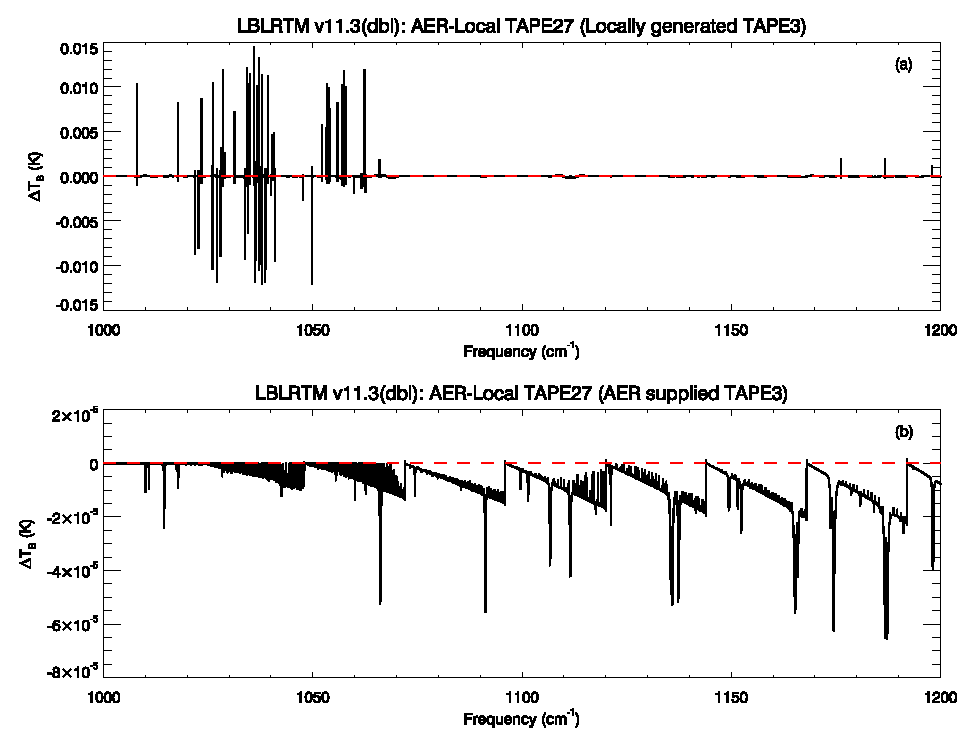
\includegraphics[bb=85 403 534 558,clip,scale=1.0]{graphics/run_example_built_in_atm_upwelling/dbl_ibm.eps}
  \qquad\textsf{LBLRTM v11.3 brightness temperature difference using AER TAPE3}\\
  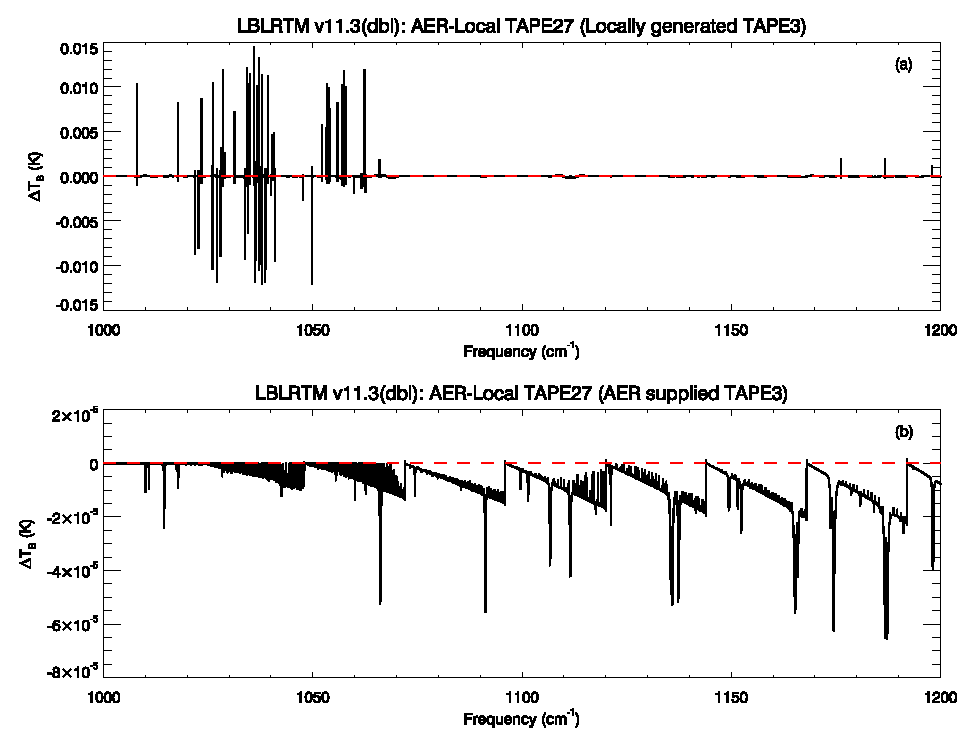
\includegraphics[bb=85 226 534 381,clip,scale=1.0]{graphics/run_example_built_in_atm_upwelling/dbl_ibm.eps}
  \caption{Built-in Atmosphere Test: Comparison of the AER-supplied \texttt{TAPE27\_ex} output to the locally generated \texttt{TAPE27} output for the \textsl{double precision} version of LBLRTM v11.3 running on an IBM AIX system. \mbox{\textbf{(a)} Using} a locally generated big-endian \texttt{TAPE3} spectroscopic datafile. \mbox{\textbf{(b)} Using} the AER-supplied big-endian \texttt{TAPE3} spectroscopic datafile.}
  \label{fig:run_example_built_in_atm_upwelling-dbl_ibm}
\end{figure}

Comparison with the same results for the linux system (figure \ref{fig:run_example_built_in_atm_upwelling-dbl}) shows no ``linear ramp'' residual feature. For the locally generated \texttt{TAPE3} case of figure \ref{fig:run_example_built_in_atm_upwelling-dbl_ibm}(a), the scattered ``line'' differences are almost the same as those seen on in the linux system results of figure \ref{fig:run_example_built_in_atm_upwelling-dbl}(a), and the periodic residuals in \ref{fig:run_example_built_in_atm_upwelling-dbl_ibm}(b) are similar to those highlighted in figure \ref{fig:run_example_built_in_atm_upwelling-dbl_1025-1200} for the linux case.


\subsection{Single precision results}
%------------------------------------
The single precision results for both the linux and AIX systems for the built-in atmosphere test case are shown in figures \ref{fig:run_example_built_in_atm_upwelling-sgl} and \ref{fig:run_example_built_in_atm_upwelling-sgl_ibm} respectively. The two sets of results are effectively identical.

The size of the residuals are, however, slightly disconcerting. These residuals are determined from comparison between the AER-supplied double precision \texttt{TAPE27\_ex} result and the locally generated \texttt{TAPE27} result using a single precision build of LBLRTM v11.3.

\begin{figure}[htp]
  \centering
  \qquad\sffamily\textbf{Verification Example: Built-in Atmosphere Upwelling}\\
  \qquad\sffamily\textbf{Red Hat linux platform; single precision}\\
  \qquad\textsf{LBLRTM v11.3 brightness temperature difference using a locally generated TAPE3}\\
  \includegraphics[bb=85 403 534 558,clip,scale=1.0]{graphics/run_example_built_in_atm_upwelling/sgl.eps}
  \qquad\textsf{LBLRTM v11.3 brightness temperature difference using AER TAPE3}\\
  \includegraphics[bb=85 226 534 381,clip,scale=1.0]{graphics/run_example_built_in_atm_upwelling/sgl.eps}
  \caption{Built-in Atmosphere Test: Comparison of the AER-supplied \texttt{TAPE27\_ex} output to the locally generated \texttt{TAPE27} output for the \textsl{single precision} version of LBLRTM v11.3 running on a Red Hat linux system. \mbox{\textbf{(a)} Using} a locally generated little-endian \texttt{TAPE3} spectroscopic datafile. \mbox{\textbf{(b)} Using} the AER-supplied little-endian \texttt{TAPE3} spectroscopic datafile.}
  \label{fig:run_example_built_in_atm_upwelling-sgl}
\end{figure}

\begin{figure}[htp]
  \centering
  \qquad\sffamily\textbf{Verification Example: Built-in Atmosphere Upwelling}\\
  \qquad\sffamily\textbf{IBM AIX platform; single precision}\\
  \qquad\textsf{LBLRTM v11.3 brightness temperature difference using a locally generated TAPE3}\\
  \includegraphics[bb=85 403 534 558,clip,scale=1.0]{graphics/run_example_built_in_atm_upwelling/sgl_ibm.eps}
  \qquad\textsf{LBLRTM v11.3 brightness temperature difference using AER TAPE3}\\
  \includegraphics[bb=85 226 534 381,clip,scale=1.0]{graphics/run_example_built_in_atm_upwelling/sgl_ibm.eps}
  \caption{Built-in Atmosphere Test: Comparison of the AER-supplied \texttt{TAPE27\_ex} output to the locally generated \texttt{TAPE27} output for the \textsl{single precision} version of LBLRTM v11.3 running on an IBM AIX system. \mbox{\textbf{(a)} Using} a locally generated big-endian \texttt{TAPE3} spectroscopic datafile. \mbox{\textbf{(b)} Using} the AER-supplied big-endian \texttt{TAPE3} spectroscopic datafile.}
  \label{fig:run_example_built_in_atm_upwelling-sgl_ibm}
\end{figure}

So, what is the cause of the relatively large residuals when comparing double and single precision calculations? Magnification of any of the panels of figures \ref{fig:run_example_built_in_atm_upwelling-sgl} or \ref{fig:run_example_built_in_atm_upwelling-sgl_ibm}, as shown in figure \ref{fig:run_example_built_in_atm_upwelling-sgl_1125-1127}, reveals the answer: a frequency shift.

\begin{figure}[htp]
  \centering
  \qquad\sffamily\textbf{Verification Example: Built-in Atmosphere Upwelling}\\
  \qquad\sffamily\textbf{Red Hat linux platform; single precision}\\
  \qquad\textsf{LBLRTM v11.3 brightness temperature difference using AER TAPE3}
  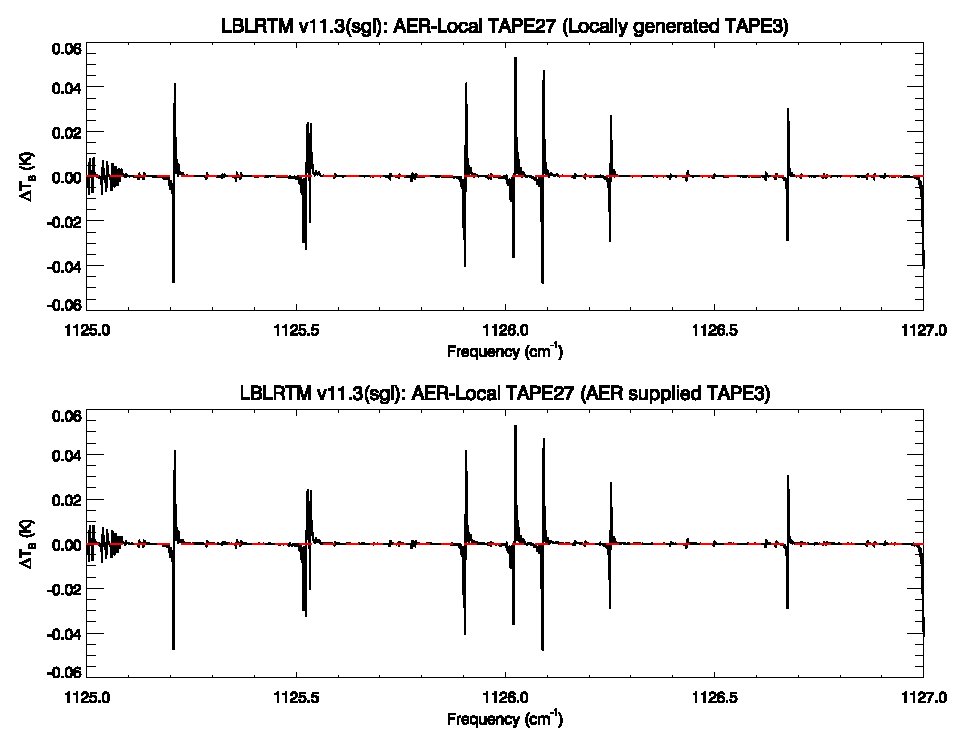
\includegraphics[bb=80 226 534 381,clip,scale=1.0]{graphics/run_example_built_in_atm_upwelling/sgl_1125-1127.eps}
  \caption{Built-in Atmosphere Test: A magnification of the 1125-1127\invcm{} spectral region from figure \ref{fig:run_example_built_in_atm_upwelling-sgl}(b) showing residuals with the characteristic shape due to a frequency shift.}
  \label{fig:run_example_built_in_atm_upwelling-sgl_1125-1127}
\end{figure}

Inspection of the \texttt{TAPE27} (radiance output) and \texttt{TAPE28} (temperature output) datafiles themselves reveals that the frequency shift is in the computed frequencies. Table \ref{tab:tape28_frequency_comparison-sgl} shows sections of computed frequency output from the AER-supplied \texttt{TAPE28\_ex} file and that from the linux system single-precision calculation \texttt{TAPE28} output file. As can be seen, the frequency grids are not the same so differenceing the two values highlights the frequency shift. The magnitude differences seen in the brightness temperatures may be quite reasonable for the frequency shift.

\begin{table}[htp]
  \centering
  \begin{tabular}{r@{.}l r@{.}l c r@{.}l r@{.}l}
    \hline
    \multicolumn{4}{c}{\sffamily\textbf{AER }\texttt{TAPE28\_ex}} & \hspace{1.0cm} & \multicolumn{4}{c}{\sffamily\textbf{Local }\texttt{TAPE28}}\\
    \multicolumn{4}{c}{\sffamily\textbf{(double precision)}} & \hspace{1.0cm} & \multicolumn{4}{c}{\sffamily\textbf{(single precision)}}\\
    \hline
    \multicolumn{2}{c}{\sffamily\textbf{Frequency}} & \multicolumn{2}{c}{\sffamily\textbf{$T_B$}} & \hspace{1.0cm} & \multicolumn{2}{c}{\sffamily\textbf{Frequency}} & \multicolumn{2}{c}{\sffamily\textbf{$T_B$}}\\
    \multicolumn{2}{c}{\sffamily\textbf{(\invcm)}} & \multicolumn{2}{c}{\sffamily\textbf{(K)}} & \hspace{1.0cm} & \multicolumn{2}{c}{\sffamily\textbf{(\invcm)}} & \multicolumn{2}{c}{\sffamily\textbf{(K)}}\\     \hline\hline
     1000&00000000 & 285&17976 & \hspace{1.0cm} & 1000&00000000 & 285&18686 \\
     1000&00024972 & 285&37625 & \hspace{1.0cm} & 1000&00024971 & 285&38333 \\
     1000&00049944 & 285&59329 & \hspace{1.0cm} & 1000&00049942 & 285&60040 \\
     1000&00074915 & 285&78922 & \hspace{1.0cm} & 1000&00074914 & 285&79636 \\
     \multicolumn{4}{c}{\ldots} & & \multicolumn{4}{c}{\ldots}\\
     1099&99958543 & 291&95654 & \hspace{1.0cm} & 1099&99963348 & 291&95667 \\ 
     1099&99983515 & 291&95805 & \hspace{1.0cm} & 1099&99988322 & 291&95816 \\ 
     1100&00008487 & 291&95968 & \hspace{1.0cm} & 1100&00013296 & 291&95975 \\ 
     1100&00033458 & 291&96149 & \hspace{1.0cm} & 1100&00038269 & 291&96158 \\
     \multicolumn{4}{c}{\ldots} & & \multicolumn{4}{c}{\ldots}\\
     1199&99917086 & 292&68271 & \hspace{1.0cm} & 1199&99912876 & 292&68265 \\ 
     1199&99942058 & 292&68505 & \hspace{1.0cm} & 1199&99937849 & 292&68506 \\ 
     1199&99967029 & 292&68725 & \hspace{1.0cm} & 1199&99962822 & 292&68732 \\ 
     1199&99992001 & 292&68910 & \hspace{1.0cm} & 1199&99987795 & 292&68921 \\ 
    \hline
  \end{tabular}
  \caption{Built-in Atmosphere Test: Comparison of tabulated frequencies and brightness temperatures between the AER-supplied \texttt{TAPE28\_ex} output file (calculated in double precision) and the local \texttt{TAPE28} output file (calculated in single precision). The difference in the frequencies, which should always be computed in double precision, is evident.}
  \label{tab:tape28_frequency_comparison-sgl}
\end{table}

This frequency shift was unexpected  since the frequency variables in the LBLRTM source code are always typed as double precision regardless of the compilation switches -- it is conceivable that at some point in the source code, an intermediate frequency calculation involves a default type floating point real variable or literal constant leading to a slight loss in precision for all subsequent calculations. The actual frequency shift spectrum between the double- and single-precision LBLRTM runs is shown in figure \ref{fig:run_example_built_in_atm_upwelling-dbl-sgl_df}.

\begin{figure}[htp]
  \centering
  \qquad\sffamily\textbf{Verification Example: Built-in Atmosphere Upwelling}\\
  \qquad\sffamily\textbf{IBM AIX platform; single precision}\\
  \qquad\textsf{LBLRTM v11.3 double-single precision run frequency difference using AER TAPE3}\\
  \includegraphics[bb=80 403 534 558,clip,scale=1.0]{graphics/run_example_built_in_atm_upwelling/dbl-sgl_df.eps}
  \caption{Built-in Atmosphere Test: The difference in the output \texttt{TAPE27} and \texttt{TAPE28} frequencies between a double- and single-precision LBLRTM v11.3 executable.}
  \label{fig:run_example_built_in_atm_upwelling-dbl-sgl_df}
\end{figure}


\section{Test Case:User-defined Atmosphere Upwelling}
%====================================================

The user-defined atmosphere test case is sightly different for that of the built-in atmosphere in that the \texttt{TAPE5} uses defined surface emissivities and reflectivities, includes CFC profile information, and invokes the FFT scanning function.

\subsection{Double precision linux results}
%------------------------------------------
The double precision results for the linux system for the user-defined atmosphere test case are shown in figure \ref{fig:run_example_user_defined_upwelling-dbl}.

\begin{figure}[htp]
  \centering
  \qquad\sffamily\textbf{Verification Example: User-defined Atmosphere Upwelling}\\
  \qquad\sffamily\textbf{Red Hat linux platform; double precision}\\
  \qquad\textsf{LBLRTM v11.3 brightness temperature difference using a locally generated TAPE3}\\
  \includegraphics[bb=85 403 534 558,clip,scale=1.0]{graphics/run_example_user_defined_upwelling/dbl.eps}
  \qquad\textsf{LBLRTM v11.3 brightness temperature difference using AER TAPE3}\\
  \includegraphics[bb=85 226 534 381,clip,scale=1.0]{graphics/run_example_user_defined_upwelling/dbl.eps}
  \caption{User-defined Atmosphere Test: Comparison of the AER-supplied \texttt{TAPE27\_ex} output to the locally generated \texttt{TAPE27} output for the \textsl{double precision} version of LBLRTM v11.3 running on a Red Hat linux system. \mbox{\textbf{(a)} Using} a locally generated little-endian \texttt{TAPE3} spectroscopic datafile. \mbox{\textbf{(b)} Using} the AER-supplied little-endian \texttt{TAPE3} spectroscopic datafile.}
  \label{fig:run_example_user_defined_upwelling-dbl}
\end{figure}

The spectral location of the main feature in the brightness temperature differences using the locally generated \texttt{TAPE3}, figure \ref{fig:run_example_user_defined_upwelling-dbl}(a), is at approximately 800\invcm{}. There are a number of water vapour lines in that region and a reasonable hypothesis for the difference is the locally generated \texttt{TAPE3} file containing more weaker water vapour lines than in the AER-supplied \texttt{TAPE3} file; presumably the creation of the latter involved some line rejection criteria.

For the case where the AER-supplied \texttt{TAPE3} is used, figure \ref{fig:run_example_user_defined_upwelling-dbl}(b), the main residual feature is an apparent sinc function centred at 937\invcm. Note that this feature also appears at the same magnitude in figure  \ref{fig:run_example_user_defined_upwelling-dbl}(a), but it is not visible due to the larger y-axis range. It would appear there is some, admittedly very small, residual, introduced into the results due to the FFT spectral reduction modules in the linux compile.


\subsection{Double precision AIX results}
%-------------------------------------------

The double precision results for the IBM AIX system for the user-defined atmosphere test case are shown in figure \ref{fig:run_example_user_defined_upwelling-dbl_ibm}.

\begin{figure}[htp]
  \centering
  \qquad\sffamily\textbf{Verification Example: User-defined Atmosphere Upwelling}\\
  \qquad\sffamily\textbf{IBM AIX platform; double precision}\\
  \qquad\textsf{LBLRTM v11.3 brightness temperature difference using a locally generated TAPE3}\\
  \includegraphics[bb=85 403 534 558,clip,scale=1.0]{graphics/run_example_user_defined_upwelling/dbl_ibm.eps}
  \qquad\textsf{LBLRTM v11.3 brightness temperature difference using AER TAPE3}\\
  \includegraphics[bb=85 226 534 381,clip,scale=1.0]{graphics/run_example_user_defined_upwelling/dbl_ibm.eps}
  \caption{User-defined Atmosphere Test: Comparison of the AER-supplied \texttt{TAPE27\_ex} output to the locally generated \texttt{TAPE27} output for the \textsl{double precision} version of LBLRTM v11.3 running on an IBM AIX system. \mbox{\textbf{(a)} Using} a locally generated big-endian \texttt{TAPE3} spectroscopic datafile. \mbox{\textbf{(b)} Using} the AER-supplied big-endian \texttt{TAPE3} spectroscopic datafile.}
  \label{fig:run_example_user_defined_upwelling-dbl_ibm}
\end{figure}

The brightness temperature differences from the run using the locally generated \texttt{TAPE3} file, figure \ref{fig:run_example_user_defined_upwelling-dbl_ibm}(a), shows the same feature as seen in  the linux system test, figure \ref{fig:run_example_user_defined_upwelling-dbl}(a).

The clear sinc function residual seen in the linux run using the AER-supplied \texttt{TAPE3} file is not present in the AIX run of figure \ref{fig:run_example_user_defined_upwelling-dbl_ibm}(b). There are other very small residual features present, but no magnification of the results indicate the presence of a residual sinc from the FFT scan function. The author is unfamiliar with that portion of the LBLRTM source code so no hypothesis as to its cause in the linux run is offered here.


\subsection{Single precision run results}
%----------------------------------------

The single precision results for both the linux and AIX systems for the user-supplied atmosphere test case are shown in figures \ref{fig:run_example_user_defined_upwelling-sgl} and \ref{fig:run_example_user_defined_upwelling-sgl_ibm} respectively.

\begin{figure}[htp]
  \centering
  \qquad\sffamily\textbf{Verification Example: User-defined Atmosphere Upwelling}\\
  \qquad\sffamily\textbf{Red Hat linux platform; single precision}\\
  \qquad\textsf{LBLRTM v11.3 brightness temperature difference using a locally generated TAPE3}\\
  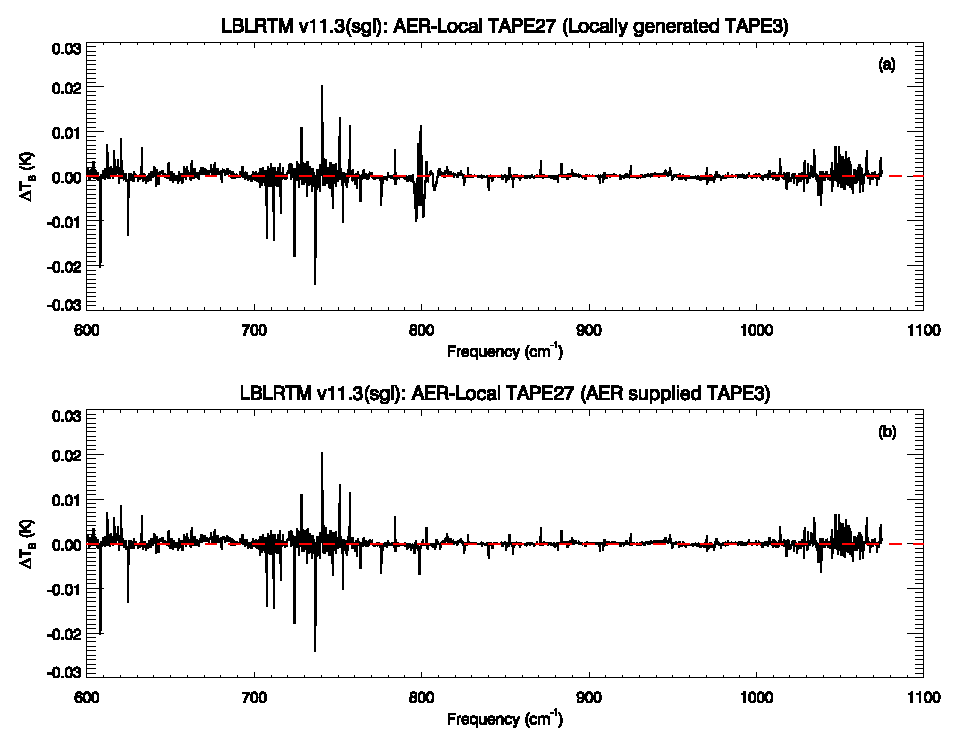
\includegraphics[bb=85 403 534 558,clip,scale=1.0]{graphics/run_example_user_defined_upwelling/sgl.eps}
  \qquad\textsf{LBLRTM v11.3 brightness temperature difference using AER TAPE3}\\
  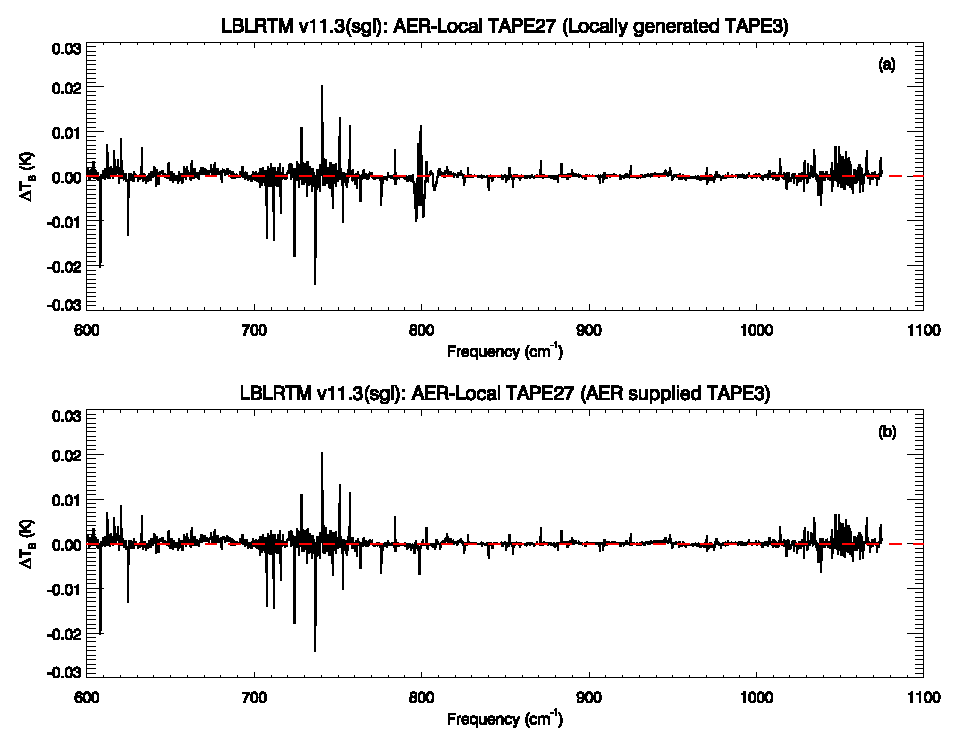
\includegraphics[bb=85 226 534 381,clip,scale=1.0]{graphics/run_example_user_defined_upwelling/sgl.eps}
  \caption{User-defined Atmosphere Test: Comparison of the AER-supplied \texttt{TAPE27\_ex} output to the locally generated \texttt{TAPE27} output for the \textsl{single precision} version of LBLRTM v11.3 running on a Red Hat linux system. \mbox{\textbf{(a)} Using} a locally generated little-endian \texttt{TAPE3} spectroscopic datafile. \mbox{\textbf{(b)} Using} the AER-supplied little-endian \texttt{TAPE3} spectroscopic datafile.}
  \label{fig:run_example_user_defined_upwelling-sgl}
\end{figure}

\begin{figure}[htp]
  \centering
  \qquad\sffamily\textbf{Verification Example: User-defined Atmosphere Upwelling}\\
  \qquad\sffamily\textbf{IBM AIX platform; single precision}\\
  \qquad\textsf{LBLRTM v11.3 brightness temperature difference using a locally generated TAPE3}\\
  \includegraphics[bb=85 403 534 558,clip,scale=1.0]{graphics/run_example_user_defined_upwelling/sgl_ibm.eps}
  \qquad\textsf{LBLRTM v11.3 brightness temperature difference using AER TAPE3}\\
  \includegraphics[bb=85 226 534 381,clip,scale=1.0]{graphics/run_example_user_defined_upwelling/sgl_ibm.eps}
  \caption{User-defined Atmosphere Test: Comparison of the AER-supplied \texttt{TAPE27\_ex} output to the locally generated \texttt{TAPE27} output for the \textsl{single precision} version of LBLRTM v11.3 running on an IBM AIX system. \mbox{\textbf{(a)} Using} a locally generated big-endian \texttt{TAPE3} spectroscopic datafile. \mbox{\textbf{(b)} Using} the AER-supplied big-endian \texttt{TAPE3} spectroscopic datafile.}
  \label{fig:run_example_user_defined_upwelling-sgl_ibm}
\end{figure}

The feature due to using the locally generated \texttt{TAPE3} file is present at around 800\invcm{} in both the linux and AIX runs. However, other than that, the two platforms yield very similar results. The character of the single precision residuals for this case are also different. Recall that the built-in atmosphere test case residuals for the single precision test case (see section \ref{sec:built_in_sgl}) indicated there was a frequency shift in the output \texttt{TAPE27} data files. That is not the case here. A magnification of figure \ref{fig:run_example_user_defined_upwelling-sgl}(b) is shown in figure \ref{fig:run_example_user_defined_upwelling-sgl_900-1000}. The character of the residuals does not indicate an issues with the \texttt{TAPE27} frequency values. This is not entirely unexpected since, if the frequency shift in the built-in atmosphere single precision test case is due to some intermediate computation at low precision, it would likely be ``removed'' -- or at least diminished -- for this test case due to the FFT scan of the high resolution result.

\begin{figure}[htp]
  \centering
  \qquad\sffamily\textbf{Verification Example: User-define Atmosphere Upwelling}\\
  \qquad\sffamily\textbf{Red Hat linux platform; single precision}\\
  \qquad\textsf{LBLRTM v11.3 brightness temperature difference using AER TAPE3}
  \includegraphics[bb=80 226 534 381,clip,scale=1.0]{graphics/run_example_user_defined_upwelling/sgl_900-1000.eps}
  \caption{User-defined Atmosphere Test: A magnification of the 900-1100\invcm{} spectral region from figure \ref{fig:run_example_user_defined_upwelling-sgl}(b). The character of the differences does not indicate a frequency shift (as seem in the figure \ref{fig:run_example_built_in_atm_upwelling-sgl_1125-1127}).}
  \label{fig:run_example_user_defined_upwelling-sgl_900-1000}
\end{figure}


\section*{Acknowledgements}
%==========================
The LBLRTM software and associated data files are an integral part of our ability to use satellite radiances in the data assimilation systems at NCEP/EMC/JCSDA. So, thanks go to the people at AER, Inc. who provide and, importantly, maintain the LBLRTM source code and spectroscopic data inputs. Any list of inidividuals would be woefully short and incomplete but special thanks go to Jean-Luc Moncet, Vivienne Payne, and Mark Shephard of AER Inc., and Tony Clough of Clough Associates for their help.

% Appendix section
%=================
\begin{appendix}
  \section{Anomalous Test Case Result with the gfortran Compiler}
%==============================================================
\label{app:busted_gfortran_compiler_results}
This section briefly details the results for the LBLRTM v11.3 built-in atmosphere test case when the gfortran v4.4.0(20081021) compiler is used with either the \texttt{-O2} or \texttt{-O3} optimisation switch. The anomalous LBLRTM v11.3 results occur for this compiler version in both the single and double precision builds, but the anomalous residuals in the single precision case are masked by the larger signal.

The double precision results for the linux/gfortran system with the optimisation switch set for the built-in atmosphere test case are shown in figure \ref{fig:run_example_built_in_atm_upwelling-dbl_gfortran_-O3}. Residuals for LBLRTM runs using the local, LNFL, and AER \texttt{TAPE3} spectroscopic input files are shown.
 
\begin{figure}[htp]
  \centering
  \qquad\sffamily\textbf{Verification Example: Built-in Atmosphere Upwelling}\\
  \qquad\sffamily\textbf{Red Hat linux platform; gfortran(\texttt{-O3}); double precision}\\
  \qquad\textsf{LBLRTM v11.3 brightness temperature difference for \textbf{Local} \texttt{TAPE3} run}\\
  \includegraphics[bb=85 490 534 648,clip,scale=1.0]{graphics/run_example_built_in_atm_upwelling/gfortran/dbl_-O3.eps}
  \qquad\textsf{LBLRTM v11.3 brightness temperature difference for \textbf{LNFL} \texttt{TAPE3} run}\\
  \includegraphics[bb=85 313 534 472,clip,scale=1.0]{graphics/run_example_built_in_atm_upwelling/gfortran/dbl_-O3.eps}
  \qquad\textsf{LBLRTM v11.3 brightness temperature difference for \textbf{AER} \texttt{TAPE3} run}\\
  \includegraphics[bb=85 138 534 296,clip,scale=1.0]{graphics/run_example_built_in_atm_upwelling/gfortran/dbl_-O3.eps}
  \caption{Built-in Atmosphere Test: Comparison of the AER-supplied \texttt{TAPE27\_ex} output to the locally generated \texttt{TAPE27} output for the \textsl{double precision} version of LBLRTM v11.3 running on a Red Hat linux system using the gfortran compiler with an optimisation level of \texttt{-O3}. \mbox{\textbf{(a)} Using} the little-endian \texttt{TAPE3} spectroscopic datafile generated from the local input shown in figure \ref{fig:local_tape3_tape5}. \mbox{\textbf{(b)} Using} the little-endian \texttt{TAPE3} spectroscopic datafile generated from the LNFL v2.5 distribution input shown in figure \ref{fig:lnfl_ex_tape3_tape5}. \mbox{\textbf{(c)} Using} the AER-supplied little-endian \texttt{TAPE3} spectroscopic datafile.}
  \label{fig:run_example_built_in_atm_upwelling-dbl_gfortran_-O3}
\end{figure}

The most obvious feature in the brightness temperature differences of figure \ref{fig:run_example_built_in_atm_upwelling-dbl_gfortran_-O3} is the ``linear ramp'' from 1000 to approximately 1025\invcm. A magnification of this spectral region is shown in figure \ref{fig:run_example_built_in_atm_upwelling-dbl_gfortran_-O3_1000-1025}. It is present regardless of which input spectroscopic \texttt{TAPE3} file is used. Additionally, after repeating the computations several times, it seems that the magnitude of this feature varies according to the compute load of the test platform. For example, the peak value of this feature at 1000\invcm{} \textit{for any of the \texttt{TAPE3} test runs} varied from -0.005 to -0.03K. 

\begin{figure}[htp]
  \centering
  \qquad\sffamily\textbf{Verification Example: Built-in Atmosphere Upwelling}\\
  \qquad\sffamily\textbf{Red Hat linux platform; gfortran(\texttt{-O3}); double precision}\\
  \qquad\textsf{LBLRTM v11.3 brightness temperature difference for \textbf{Local} \texttt{TAPE3} run}\\
  \includegraphics[bb=85 490 534 648,clip,scale=1.0]{graphics/run_example_built_in_atm_upwelling/gfortran/dbl_-O3_1000-1025.eps}
  \qquad\textsf{LBLRTM v11.3 brightness temperature difference for \textbf{LNFL} \texttt{TAPE3} run}\\
  \includegraphics[bb=85 313 534 472,clip,scale=1.0]{graphics/run_example_built_in_atm_upwelling/gfortran/dbl_-O3_1000-1025.eps}
  \qquad\textsf{LBLRTM v11.3 brightness temperature difference for \textbf{AER} \texttt{TAPE3} run}\\
  \includegraphics[bb=85 138 534 296,clip,scale=1.0]{graphics/run_example_built_in_atm_upwelling/gfortran/dbl_-O3_1000-1025.eps}
  \caption{Built-in Atmosphere Test: A magnification of the 1000-1025\invcm{} spectral region from figure \ref{fig:run_example_built_in_atm_upwelling-dbl_gfortran_-O3}. \mbox{\textbf{(a)} Using} the little-endian \texttt{TAPE3} spectroscopic datafile generated from the local input shown in figure \ref{fig:local_tape3_tape5}. \mbox{\textbf{(b)} Using} the little-endian \texttt{TAPE3} spectroscopic datafile generated from the LNFL v2.5 distribution input shown in figure \ref{fig:lnfl_ex_tape3_tape5}. \mbox{\textbf{(c)} Using} the AER-supplied little-endian \texttt{TAPE3} spectroscopic datafile.}
  \label{fig:run_example_built_in_atm_upwelling-dbl_gfortran_-O3_1000-1025}
\end{figure}

  \section{Anomalous Test Case Result with IBM Compiler}
%=====================================================
\label{app:busted_ibm_compiler_results}
This section briefly details the results for the LBLRTM v11.3 user-defined atmosphere test case when the IBM AIX xlf95 v10.1.0000.0002 compiler is used (henceforth referred to as v10.1.0.2) . You can find out the version of your IBM compiler via the \texttt{-qversion} switch:
\begin{verbatim}
  $ xlf95 -qversion
  IBM XL Fortran Enterprise Edition V10.1 for AIX
  Version: 10.01.0000.0002\end{verbatim}

The anomalous LBLRTM v11.3 results only occur for this compiler version and only for the double precision build -- the single precision build does not appear to have any problem. Additionally, the problem also only occurs for the user-defined atmosphere test case; the built-in atmosphere test case produces expected results for all builds using the v10.1.0.2 AIX compiler. Thus, it is thought that the anomalous results stem from some sort of interaction between the double precision build and the use of the \texttt{SCAN} options - in this particular case the \texttt{FFTSCN} option, but similar anomalous results have been seen when the \texttt{SCNMRG} option has been used.
 
\begin{figure}[htp]
  \centering
  \qquad\sffamily\textbf{Verification Example: Built-in Atmosphere Upwelling}\\
  \qquad\sffamily\textbf{IBM AIX xlf95 v10.1.0.2 compiler; double precision build}\\
  \qquad\textsf{LBLRTM v11.3 brightness temperature difference using AER TAPE3}\\
  \includegraphics[bb=80 403 534 558,clip,scale=1.0]{graphics/run_example_user_defined_upwelling/ibm/dbl-busted-dt.eps}
  \qquad\textsf{LBLRTM v11.3 brightness temperature spectra using AER TAPE3}\\
  \includegraphics[bb=80 403 534 558,clip,scale=1.0]{graphics/run_example_user_defined_upwelling/ibm/dbl-busted-t.eps}
  \caption{Comparison of the AER-supplied \texttt{TAPE27\_ex} output to the locally generated \texttt{TAPE27} output for the \textsl{double precision} version of LBLRTM v11.3 using the IBM AIX xlf 95 v10.1.0.2 compiler. The AER-supplied big-endian \texttt{TAPE3} spectroscopic datafile was used. \mbox{\textbf{(Upper Panel)} Brightness} temperature differences. \mbox{\textbf{(Lower Panel)} Brightness} temperature spectra. The locally generated result using the v10.1.0.2 compiler is clearly incorrect.}
  \label{fig:run_example_user_defined_atm_upwelling-dbl-ibm_busted}
\end{figure}


\end{appendix}

\end{document}

